Large language models~\citep{openai2023gpt4, touvron2023llama} have demonstrated remarkable performance on various natural language processing tasks. This has inspired numerous works to build speech language models~\citep{borsos2022audiolm}, which have achieved significant breakthroughs across various speech processing tasks~\citep{wang2023neural,zhang2023speechgpt, rubenstein2023audiopalm, dong2023polyvoice}. A key commonality among these works is the utilization of discrete speech representations.
Current discrete speech representations can be categorized into two types: semantic tokens and acoustic tokens~\citep{borsos2022audiolm}. Semantic tokens are typically from self-supervised pre-trained models with masked language modeling as training objective~\citep{hsu2021hubert, baevski2020wav2vec, chung2021w2vbert}. Derived through k-means clustering on representations from a specific intermediate layer, semantic tokens are depicted as sequences with one-dimensional structure.
Acoustic tokens can be extracted from neural audio codecs with reconstruction as training objective~\citep{zeghidour2021soundstream, défossez2022high}. 
Utilizing residual vector quantization~(RVQ) with hierarchical quantizers for discretization, acoustic tokens are represented as matrices consisting of two dimensions: timesteps and quantizers.
% Certain studies analysis the relationship between speech tokens and different speech attributes~\citep{sicherman2023analysing, abdullah2023information}. However, there is a lack of quantitative analysis on the information composition of different speech tokens.

However, neither of current speech tokens is specifically designed for speech language modeling, and there has been no exploration into their suitability for building speech language models.
To this end, we build Speech Language Model Token Benchmark~(\bench), to assess the suitability of speech tokens for constructing speech language models.
For speech language models, good speech tokens should possess the following two key characteristics: i)~Strong alignment with text; ii) Effective preservation of speech information. From the results on \bench, we observe that semantic tokens exhibit a high alignment with text while losing some information in speech, such as timbre. Acoustic tokens excel in preserving speech information effectively but do not demonstrate a strong alignment with text.
% We observe that semantic tokens primarily model the content information in speech while disregarding paralinguistic information. Acoustic tokens capture all aspects of information in speech, including content, timbre, prosody, recording conditions, etc. However, the information they contain is mixed together without being decoupled.
% Current speech discrete representations can be categorized into two types: semantic tokens and acoustic tokens~\citep{borsos2022audiolm}. Semantic tokens are typically derived from self-supervised pre-trained models with masked language modeling as training objective functions~\citep{hsu2021hubert, baevski2020wav2vec, chung2021w2vbert}. They primarily model the content information in speech while disregarding paralinguistic information~\citep{polyak2021speech}. Acoustic tokens can be extracted from neural audio codecs with reconstruction as training objective functions~\citep{zeghidour2021soundstream, défossez2022high}. They capture all aspects of information in speech, including content, timbre, prosody, recording conditions, etc. However, the information they contain is mixed together without being decoupled.

% \begin{figure*}[t] 
%     % \vspace{-5pt}
%     \centering 
%     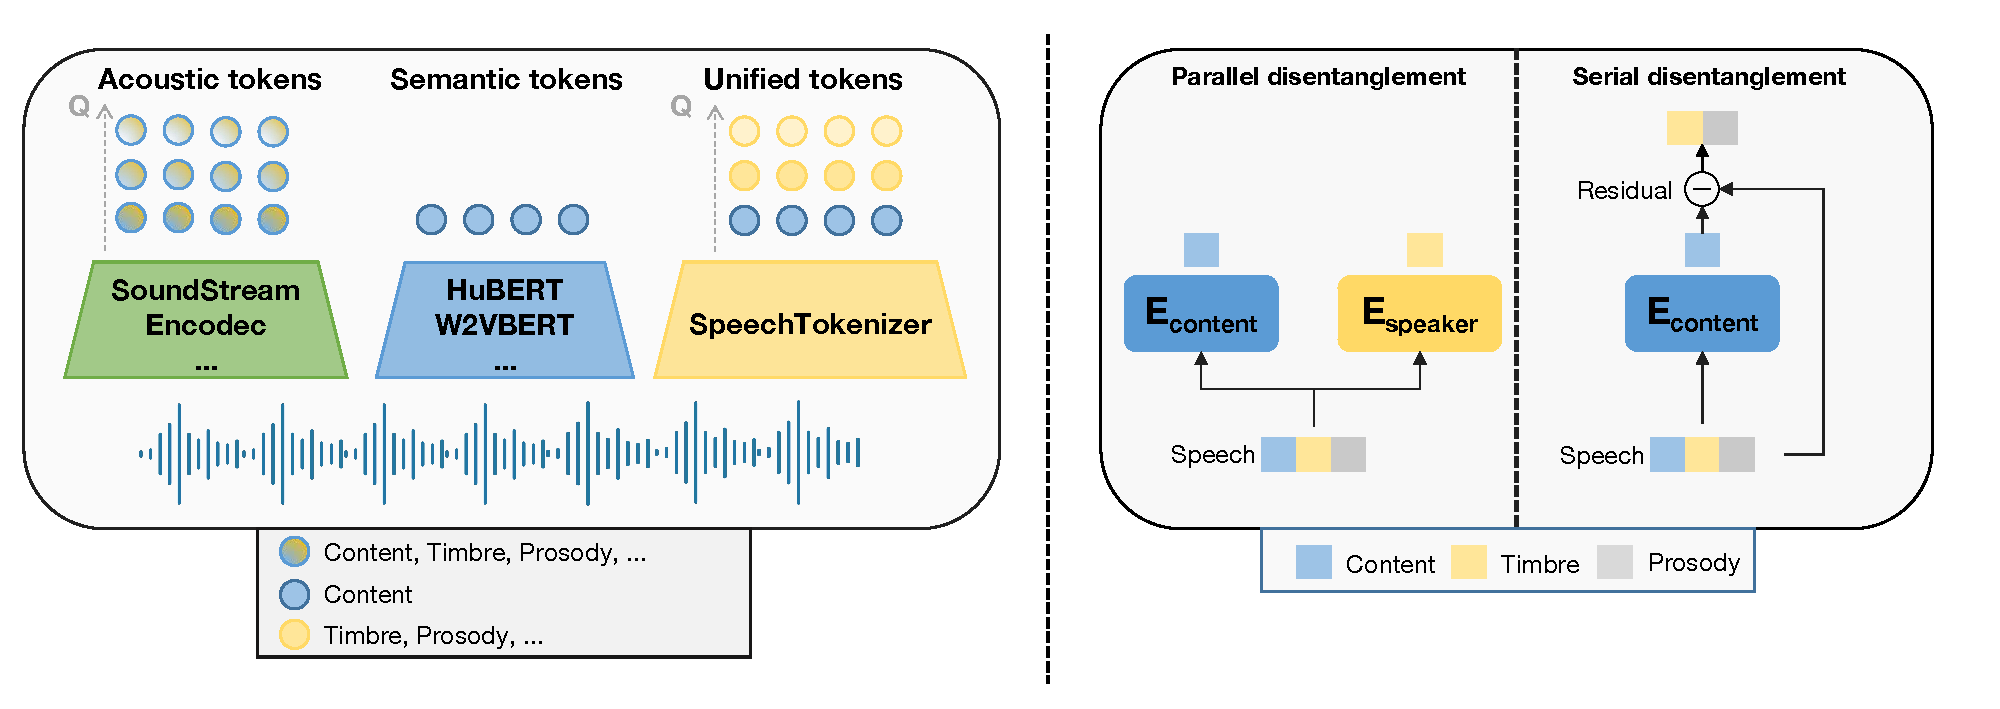
\includegraphics[width=1\textwidth]{Figures/token_disentanglement.pdf} 
%     \caption{\textbf{Left}: Illustration of information composition of different discrete speech representations. Speech tokens are represented as colored circles. \textbf{Right}: Illustration of parallel disentanglement and serial disentanglement. Speech are represented as blocks to denote their information components. $E_{content}$ denotes the content encoder; $E_{speaker}$ denotes the speaker encoder.}

%     \label{fig:token_disentangle} 
% \end{figure*}

\begin{figure*}[t] 
    % \vspace{-5pt}
    \centering 
    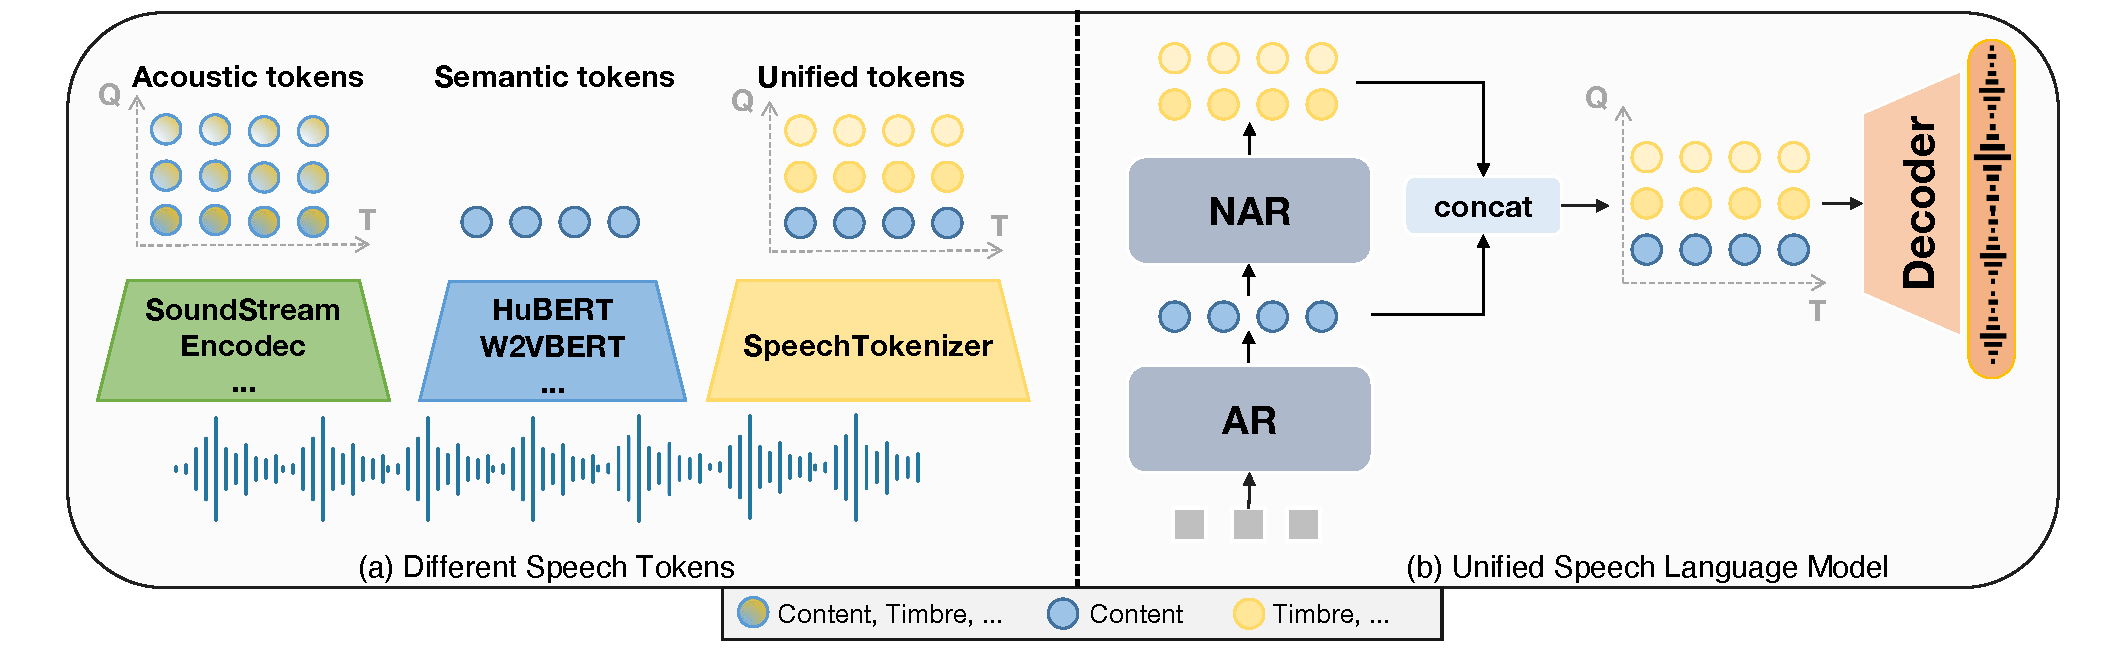
\includegraphics[width=1\textwidth]{Figures/token_model.pdf} 
    \caption{\textbf{Left}: Illustration of information composition of different discrete speech representations. \textbf{Right}: Illustration of unified speech language models. Speech tokens are represented as colored circles and different colors represent different information.}

    \label{fig:token_model} 
\end{figure*}

\begin{table*}[t]
    % \setlength{\abovecaptionskip}{-0.cm}
    \setlength{\belowcaptionskip}{-0.2cm}
    % \renewcommand{\arraystretch}{1.2}
    \Large
    \centering
    \resizebox{0.7\textwidth}{!}{
    \begin{tabular}{l|c|c|c}
        \toprule
        ~ & Accurate Content & High-quality Speech & Single Tokenzier \\
        \midrule
        Semantic LM & $\surd$ & $\times$ & $\surd$ \\
        Acoustic LM & $\times$ & $\surd$ & $\surd$ \\
        Hierarchical LM & $\surd$ & $\surd$ & $\times$ \\
        USLM~(ours) & $\surd$ & $\surd$ & $\surd$ \\
        \bottomrule
    \end{tabular}}
    \caption{Comparision between different speech language models. \textit{Semantic LM} refers to semantic language models. \textit{Acoustic LM} refers to acoustic language models. \textit{Hierarchical LM} refers to hierarchical speech language models. \textit{USLM} refers to our unified speech language model.
    }
    \label{tab:slm_comparision}
\vspace{-0.5em} 
\end{table*}

Building upon two speech tokens, there exist three modeling approaches for speech language models:
\textit{i)~Semantic language models} are constructed using semantic tokens and employ an external unit vocoder for speech synthesis.~\citep{lakhotia2021generative, zhang2023speechgpt}. While capturing semantically accurate content, their speech generation results in poor quality and a loss of acoustic details.
\textit{ii)~Acoustic language models} are built on acoustic tokens. Taking VALL-E~\citep{wang2023neural} as an example, despite achieving impressive zero-shot text-to-speech~(TTS) capabilities, it still suffers from problems like inaccurate content, due to the complex information within acoustic tokens.
\textit{iii)~Hierarchical speech language models} comprise semantic token language models and acoustic token language models, which capture content information and acoustic details respectively~\citep{borsos2022audiolm, rubenstein2023audiopalm, dong2023polyvoice}. This structure shows promising results in both content and speech quality, but the multi-stage modeling approach is more complex, leading to several drawbacks such as error accumulation and slower processing speed. Additionally, there is significant information redundancy between semantic tokens and acoustic tokens, which introduces unnecessary modeling complexities. 
To this end, we aim to unify the three modeling approaches through unifying semantic and acoustic tokens into a specialized speech tokens designed for speech language models. 
Specifically, we can conduct information disentanglement in the RVQ structure of acoustic tokens, enabling the first quantizer to generate tokens containing content information, similar to semantic tokens, while the subsequent quantizers complement the remaining paralinguistic information. 

% unifying semantic tokens and acoustic tokens.
% into one single discrete speech representation.
% and decouple the information between the two tokens, where semantic tokens contains content information and acoustic tokens serve to complement the paralinguistic information lost by semantic tokens.
% Based on the unified speech tokens, we can unify the three modeling approaches, allows for hierarchical modeling of speech without complex architecture.

% 


% VALL-E~\citep{wang2023neural} achieves impressive zero-shot text-to-speech~(TTS) capabilities by modeling text-to-acoustic tokens generation in a neural codec language model. However, acoustic tokens capture all aspects of information in speech, which increases the complexity of modeling text-to-acoustic tokens. To mitigate this information gap, SPEAR-TTS~\citep{zhang2023speak} uses semantic tokens as a bridge between text and acoustic tokens. It first generates semantic tokens from text and then produces acoustic tokens from semantic tokens. However, this multi-stage modeling approach is more complex and can lead to problems like error accumulation and slow inference speed. Moreover, there is significant information redundancy between semantic tokens and acoustic tokens, which introduces unnecessary modeling challenges. To this end, we aim to unify semantic tokens and acoustic tokens into a single discrete speech representation and decouple the information between the two tokens, where semantic tokens contains content information and acoustic tokens serve to complement the paralinguistic information lost by semantic tokens.

Speech representation disentanglement approaches mainly adopt a parallel disentanglement strategy. This entails simultaneously feeding speech into separate content encoders, speaker encoders, etc., in order to extract different representations and attain information disentanglement~\citep{qian2020unsupervised, polyak2021speech}. However, this approach heavily relies on prior knowledge and introduces strong inductive biases, leading to increased complexity and a potential oversight of certain speech information, such as prosody.
Similar to VQVC~\citep{wu2020one}, we adopt residual structure to achieve serial disentanglement of speech. For neural 
audio codec, the cumulative representations from all RVQ layers encompass all dimensions of speech information. By ensuring the first layer representations contain content-related information, the subsequent residual layers will naturally fill in the gaps with remaining details—specifically, modeling the paralinguistic information.

We propose \method, a unified speech tokenizer for speech large language models. \method adopts the Encoder-Decoder architecture with residual vector quantization.
To unify semantic and acoustic tokens, we disentangle different aspects of speech information hierarchically across different RVQ layers.
By employing a semantic teacher to guide the first RVQ quantizer, the first layer tokens can effectively capture content information. With residual structure, the subsequent quantizers complement the remaining paralinguistic information. 
Building upon \method, we build a \textbf{U}nified \textbf{S}peech \textbf{L}anguage \textbf{M}odel~(USLM) consisting
of autoregressive and non-autoregressive models. Experiments results show that \method can achieve similar performance on speech reconstruction with EnCodec, good speech disentanglement and USLM is superior to VALL-E on zero-shot TTS tasks.

% It leverages knowledge distillation to learn semantic information and utilizes residual structures to realize serial information disentanglement. \method unifies semantic tokens and acoustic tokens into a single speech discrete representation and achieves hierarchical modeling of information. Concretely, semantic tokens model content information, while acoustic tokens serve to complement the paralinguistic information lost by semantic tokens. 
% To evaluate different speech discrete representations from information perspective, we establish DSR Benchmark.


Our contributions include the following:
 \begin{itemize}[itemsep=1pt, leftmargin=10pt, parsep=0pt, topsep=1pt]
    \item 
    We propose \method, which unifies the semantic and acoustic tokens through disentangling different aspects of speech information hierarchically.


    % \item 
    % We propose a novel serial disentanglement method using residual structure.


    \item 
    We establish \bench, a  benckmark to assess the suitability of speech tokens for constructing speech language models.

    
    \item 
    We construct a unified speech language model based on \method, which outperforms VALL-E on zero-shot TTS task.


    
    
\end{itemize}
